\section{Question2}
\begin{enumerate}[a).]
\item  \textbf{algorithm description:}
\begin{itemize}
	\item first,we randomly choose $v$ from the array $A$;
	\item second,we split $A$ into three categories : elements greater than $v$,
	those equal to $v$,and those smaller than $v$.Call these $A_L,A_v,A_R$ respectively.
	\item then,we have 
	\begin{equation*}
	 \text{select}(A,k) = \left\lbrace 
	 \begin{array}{lll}
	 \text{select}(A_L,k) &\text{if}& k \leq  \text{len}(A_L)\\
	 v  &\text{if}& \text{len}(A_L) < k \leq \text{len}(A_L) + \text{len}(A_v)\\
	 \text{select}(A_R,k-\text{len}(A_L)-\text{len}(A_v)) &\text{if}& k > \text{len}(A_L) + \text{len}(A_v)
	 \end{array}
	 \right.
	\end{equation*}
	here ``len'' represents the length of an array.
\end{itemize}
pseudo-code:
\begin{algorithm}
\caption{find the $k^{th}$ largest element in an unsorted array}
\begin{algorithmic}[1]
\Require An unsorted array $A$ and $k$
\Ensure the $k^{th}$ largest number	of  $A$
\Function{select}{$A,k$}
\If {$k \leq 0$ or $k > \text{len}(A)$} 
\State \Return error
\EndIf
\State randomly choose $v$ of $A$
\State $A_L=\{\},A_v=\{\},A_R=\{\}$
\For {$i = 1 $ to $\text{len}(A)$} 
\If {$A[i] > v$}
\State $A_L = A_L \bigcup \{A[i]\} $
\ElsIf {$A[i] = v$}
\State $A_v = A_v \bigcup \{A[i]\} $
\Else
\State $A_R = A_R \bigcup \{A[i]\} $
\EndIf
\EndFor
\If {$k \leq \text{len}(A_L)$}
\State \Return \Call{select}{$A_L,k$}
\ElsIf {$k \leq \text{len}(A_L) + \text{len}(A_v)$}
\State \Return $v$ 
\Else
\State \Return \Call{select}{$A_R,k- \text{len}(A_L) - \text{len}(A_v)$}
\EndIf
\EndFunction
\end{algorithmic}
\end{algorithm}
\item  \textbf{subproblem reduction graph}
\begin{figure}[H]
\centering
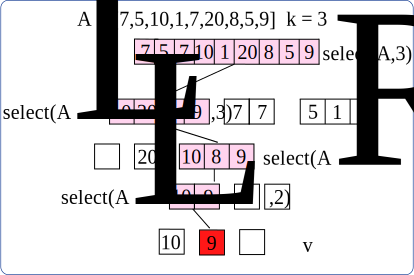
\includegraphics[width = 0.6\textwidth,height=0.25\textheight]{pictures/graph1}
\caption{problem instance}
\end{figure}
\item \textbf{proof of the correctness} \\
In terms of the input constraints, it should throw an exception given $k \leq 0 $ or $k > \text{len}(A)$.
What we want is finding the $k^{th}$ largest number of array $A$,there is no need to sort the array.
In every recursion, the search can be narrowed down to one of three sublists until we choose the correct one of 
singletons.

\item \textbf{complexity of the algorithm} \\
Splitting $A$ into three parts costs linear time.
\begin{itemize}
	\item The most worst situation is that we choose the smallest  number every times,
	then it would force our algorithm to perform \\
	\[
	T(n) = T(n-1) + O(n)
	\]
	or $O(n^{2})$ operations.
	\item The best-case scenario is that we select the median at each iteration,
	thus it would perform \\
	\[
	T(n) = T(n/2) + O(n) 
	\]
	or $O(n)$ operations.
	\item good choice: select a nearly-central element ,
		$\text{len}(A_L) \geq \epsilon \text{len}(A)$,$
		\text{len}(A_R) \geq \epsilon \text{len}(A)$ for a fixed $0 < \epsilon < 1$,
	\begin{align*}
	T(n) \leq &T((1-\epsilon)\text{len}(A)) + O(n) \\
	 \leq &cn + c(1-\epsilon)n + c(1-\epsilon)^{2}n + ... \\
	 =& O(n)
	\end{align*}	
			
	
\end{itemize} 




\end{enumerate}	
	
